\chapter{Implementation, Testing, and Results}
%%%%%%%%%%%%%%%%%%%%%%%%%%%%%%%%%%%%%%%%%
\section{Introduction}
This chapter covers the implementation stack, functional features, testing strategy, comparison with other systems, and complexity analysis of \projname{}.

%%%%%%%%%%%%%%%%%%%%%%%%%%%%%%%%%%%%%%%%%
\section{Language and Runtime}
%%%%%%%%%%%%%%%%%%%%%%%%%%%%%%%%%%%%%%%%%
The application is implemented in Java \index{Java} \cite{oaks_java_security}. Java provides portability, rich library support, and strong ecosystem compatibility with desktop application development.

%%%%%%%%%%%%%%%%%%%%%%%%%%%%%%%%%%%%%%%%%
\section{User Interface}
%%%%%%%%%%%%%%%%%%%%%%%%%%%%%%%%%%%%%%%%%
JavaFX \index{JavaFX} \cite{javafx} is used for the desktop UI. It supports modern interface rendering, event handling, and structured layout without requiring platform-specific UI code.

%%%%%%%%%%%%%%%%%%%%%%%%%%%%%%%%%%%%%%%%%
\section{Application UI Flow}
%%%%%%%%%%%%%%%%%%%%%%%%%%%%%%%%%%%%%%%%%
The application presents a structured user interface that guides the user through vault operations. The UI flow consists of three primary screens: vault creation/login, vault file browser, and import/export dialogs.

\subsection{Vault Creation and Login Screen}
The initial screen allows the user to either create a new vault or open an existing one. During vault creation, the user provides a password which is validated using the built-in password strength checker. The password strength indicator provides real-time feedback to help users choose strong vault passwords. Once a vault is created or opened, the user is directed to the main vault file browser. The vault creation screen is shown in Figure \ref{fig:ui_vault_creation}.

\begin{figure}[h]
	\centering
	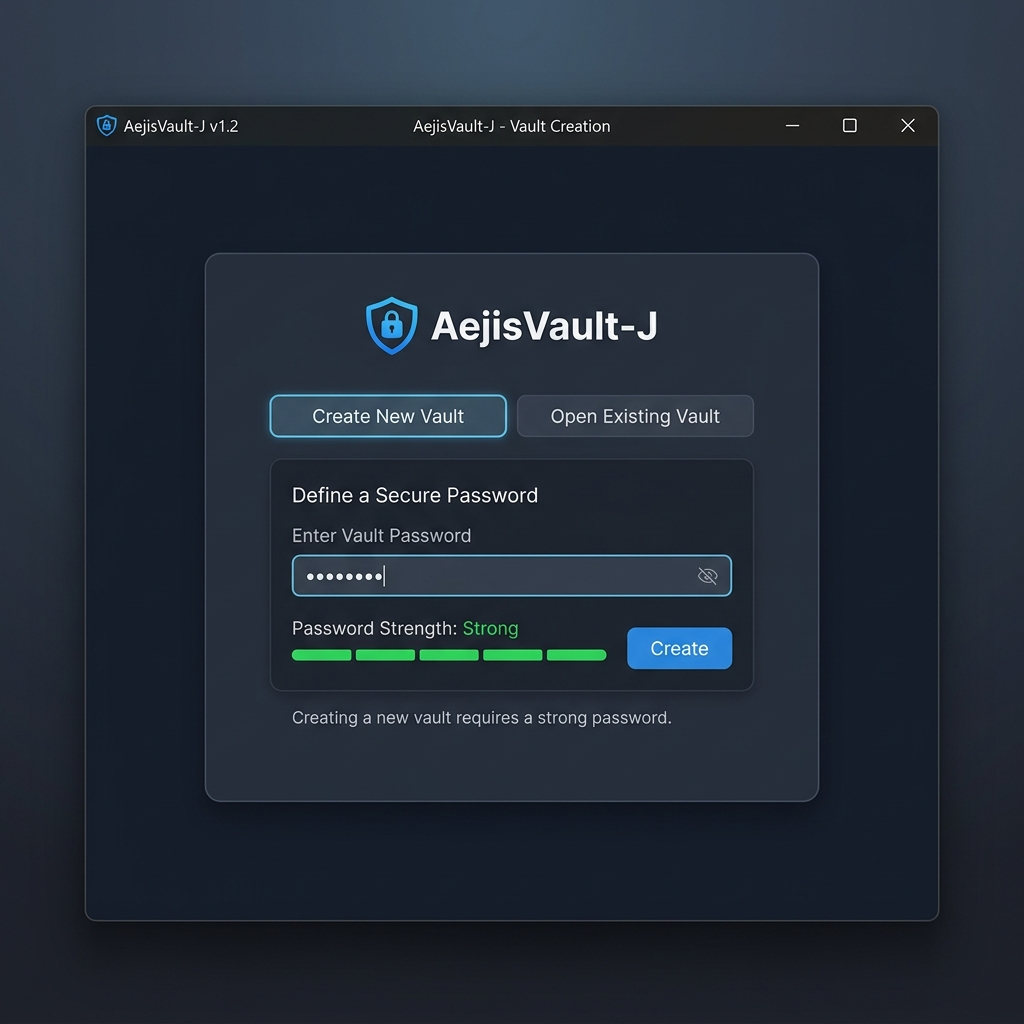
\includegraphics [width=0.75\textwidth] {figures/ui_vault_creation}
	\caption{Vault creation and login screen of \projname{}. Users can create a new vault or open an existing one with password authentication.}
	\label{fig:ui_vault_creation}	
\end{figure}

\subsection{Main Vault File Browser}
After successful authentication, the user is presented with the main vault file browser interface. The left panel displays the folder hierarchy within the vault, and the right panel shows the contents of the selected folder. The toolbar provides access to core operations: importing files, exporting files, creating new folders, deleting items, locking the vault, and accessing settings. The vault file browser is shown in Figure \ref{fig:ui_file_browser}.

\begin{figure}[h]
	\centering
	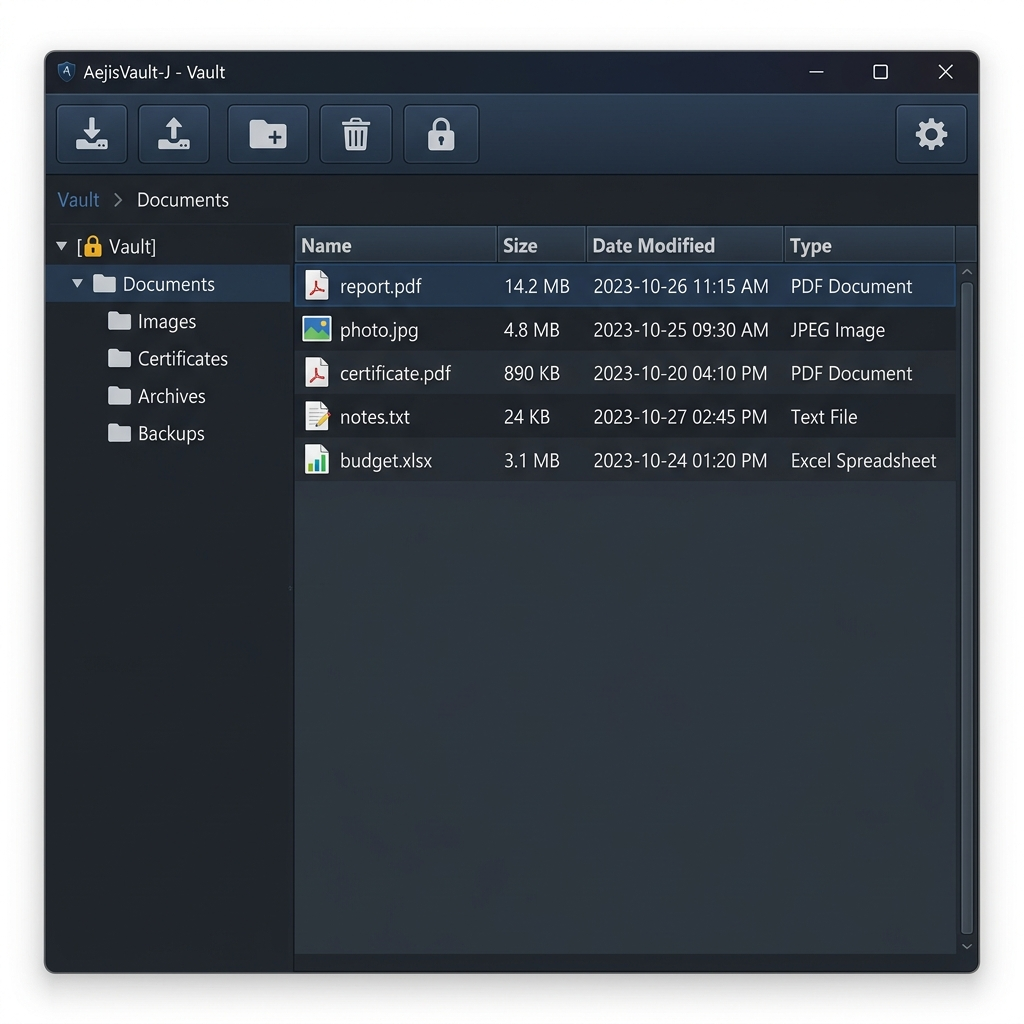
\includegraphics [width=0.75\textwidth] {figures/ui_file_browser}
	\caption{Main vault file browser of \projname{}. The interface provides a familiar file manager layout with vault-specific operations in the toolbar.}
	\label{fig:ui_file_browser}	
\end{figure}

\subsection{Import and Export Operations}
The import dialog allows users to select files from the host filesystem and encrypt them into the vault. A progress indicator shows the encryption status during the import process. The export dialog similarly allows users to select vault items and decrypt them to the host filesystem, with an explicit warning that exported files will no longer be protected by the vault. The import dialog is shown in Figure \ref{fig:ui_import_export}.

\begin{figure}[h]
	\centering
	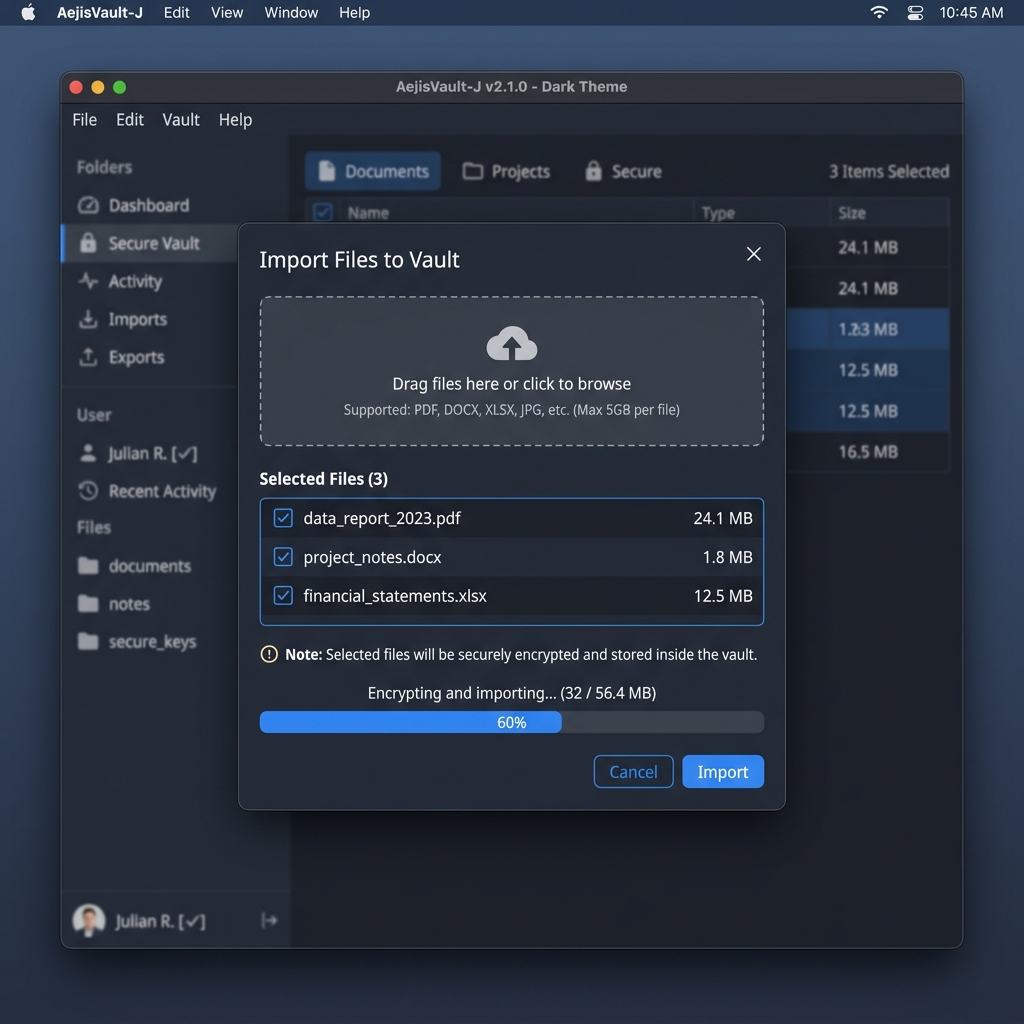
\includegraphics [width=0.75\textwidth] {figures/ui_import_export}
	\caption{Import/Export dialog of \projname{}. The interface shows file selection, encryption progress, and security warnings for export operations.}
	\label{fig:ui_import_export}	
\end{figure}

%%%%%%%%%%%%%%%%%%%%%%%%%%%%%%%%%%%%%%%%%
\section{Cryptographic Libraries}
%%%%%%%%%%%%%%%%%%%%%%%%%%%%%%%%%%%%%%%%%
The project uses \texttt{javax.crypto} alongside BouncyCastle \index{BouncyCastle} \cite{bouncycastle} for cryptographic operations. This combination allows access to standard Java cryptography APIs and supplemental algorithm support where needed.

%%%%%%%%%%%%%%%%%%%%%%%%%%%%%%%%%%%%%%%%%
\section{Build and Packaging}
%%%%%%%%%%%%%%%%%%%%%%%%%%%%%%%%%%%%%%%%%
Gradle \index{Gradle} manages the build process, dependency resolution, and packaging tasks. The project can be targeted for native distribution formats such as Windows \texttt{.exe}, Linux AppImage, and macOS \texttt{.app}.

%%%%%%%%%%%%%%%%%%%%%%%%%%%%%%%%%%%%%%%%%
\section{Vault Lifecycle}
%%%%%%%%%%%%%%%%%%%%%%%%%%%%%%%%%%%%%%%%%
The system supports vault creation and opening. During creation, the vault structure is initialized, and the encrypted key material is stored. During opening, the password-based key derivation process is performed and the vault contents are decrypted if authentication succeeds.

%%%%%%%%%%%%%%%%%%%%%%%%%%%%%%%%%%%%%%%%%
\section{Import and Export Operations}
%%%%%%%%%%%%%%%%%%%%%%%%%%%%%%%%%%%%%%%%%
Import operations copy files or folders into the vault. Export operations copy selected items out of the vault to a chosen host path. Since export means leaving the protected environment, the system marks this as an explicit trust boundary.

%%%%%%%%%%%%%%%%%%%%%%%%%%%%%%%%%%%%%%%%%
\section{Folder Hierarchy Management}
%%%%%%%%%%%%%%%%%%%%%%%%%%%%%%%%%%%%%%%%%
The vault preserves an internal folder tree. This helps users organize content in a way that resembles a normal file manager while still keeping the data inside the encrypted container.

%%%%%%%%%%%%%%%%%%%%%%%%%%%%%%%%%%%%%%%%%
\section{Password Change}
%%%%%%%%%%%%%%%%%%%%%%%%%%%%%%%%%%%%%%%%%
The password change feature rewraps the \mvk{} with a new \kek{} derived from the new password. This design avoids re-encrypting every file in the vault and reduces the risk and cost of password updates.

%%%%%%%%%%%%%%%%%%%%%%%%%%%%%%%%%%%%%%%%%
\section{Backup Utility}
%%%%%%%%%%%%%%%%%%%%%%%%%%%%%%%%%%%%%%%%%
Backup support helps users preserve encrypted vault copies. Since the vault file is self-contained, backups can be made at the container level rather than by copying many individual files.

%%%%%%%%%%%%%%%%%%%%%%%%%%%%%%%%%%%%%%%%%
\section{Password Strength Checker}
%%%%%%%%%%%%%%%%%%%%%%%%%%%%%%%%%%%%%%%%%
The password strength checker offers immediate feedback on likely weakness patterns such as short length or common structure. It does not replace cryptographic protection, but it helps improve user behavior.

%%%%%%%%%%%%%%%%%%%%%%%%%%%%%%%%%%%%%%%%%
\section{Unit Testing Strategy}
%%%%%%%%%%%%%%%%%%%%%%%%%%%%%%%%%%%%%%%%%
The project includes more than 80 unit tests spanning cryptography, virtual file system logic, container serialization, and service-layer behavior. Comprehensive testing is important because security code frequently fails in edge cases.

%%%%%%%%%%%%%%%%%%%%%%%%%%%%%%%%%%%%%%%%%
\section{Coverage Areas}
%%%%%%%%%%%%%%%%%%%%%%%%%%%%%%%%%%%%%%%%%
The tests cover:
\begin{itemize}
  \item encryption and decryption correctness,
  \item wrong-password handling,
  \item container read/write behavior,
  \item folder and file tree logic,
  \item service-layer state transitions,
  \item password-change operations,
  \item auto-lock behavior and warnings.
\end{itemize}

%%%%%%%%%%%%%%%%%%%%%%%%%%%%%%%%%%%%%%%%%
\section{Security Audit Summary}
%%%%%%%%%%%%%%%%%%%%%%%%%%%%%%%%%%%%%%%%%
A security audit was completed and did not identify critical vulnerabilities in the design as implemented. This does not mean the system is invulnerable; rather, it indicates that no severe issues were found within the examined scope and assumptions.

%%%%%%%%%%%%%%%%%%%%%%%%%%%%%%%%%%%%%%%%%
\section{Observed JVM Limitations}
%%%%%%%%%%%%%%%%%%%%%%%%%%%%%%%%%%%%%%%%%
The audit identified some practical limitations inherited from the runtime environment:
\begin{itemize}
  \item Java password input components may internally use \texttt{String} representations.
  \item Memory zeroing cannot be absolutely guaranteed for all intermediate copies.
  \item Encoding and framework operations may create temporary data copies.
\end{itemize}
These observations are important because they prevent overstatement of memory hygiene guarantees.

%%%%%%%%%%%%%%%%%%%%%%%%%%%%%%%%%%%%%%%%%
\section{Comparison with VeraCrypt}
%%%%%%%%%%%%%%%%%%%%%%%%%%%%%%%%%%%%%%%%%
VeraCrypt \index{VeraCrypt} \cite{veracrypt} is a mature disk and volume encryption tool with kernel-level integration and broad system protection. \projname{} differs in that it is Java-only, application-level, and centered on an explicit import/export model. This makes it simpler to understand for controlled workflows, though it does not offer the same class of system-wide protection.

%%%%%%%%%%%%%%%%%%%%%%%%%%%%%%%%%%%%%%%%%
\section{Comparison with Disk Encryption}
%%%%%%%%%%%%%%%%%%%%%%%%%%%%%%%%%%%%%%%%%
Disk encryption protects the entire system volume. \projname{} protects selected files only. This narrower scope gives the user more flexibility and portability, but it also means that protection is limited to the vault boundary.

\begin{table}[h]
\centering
\caption{Comparison of \projname{} with common alternatives}
\begingroup
\renewcommand{\arraystretch}{1.3}
\begin{tabular}{l l l l}
\hline
\rowcolor[HTML]{67FD9A}
{\bfseries Feature} & {\bfseries AegisVault-J} & {\bfseries VeraCrypt} & {\bfseries Disk Encryption} \\
\hline
\rowcolor[HTML]{EFEFEF}
Protection scope & Selected files & Volumes/containers & Entire disk/system \\
\hline
User model & Import/export & Mounted/container & Transparent \\
\hline
\rowcolor[HTML]{EFEFEF}
Platform & Java application & Native integration & OS-level \\
\hline
Portability & High & High to moderate & Low to moderate \\
\hline
\rowcolor[HTML]{EFEFEF}
Granularity & File-level control & Volume-level & Whole-device \\
\hline
Kernel dependency & None & Low-level & High \\
\hline
\end{tabular}
\endgroup
\label{tab:comparison}
\end{table}

%%%%%%%%%%%%%%%%%%%%%%%%%%%%%%%%%%%%%%%%%
\section{Technical Complexity}
%%%%%%%%%%%%%%%%%%%%%%%%%%%%%%%%%%%%%%%%%
The project combines several advanced topics: cryptography, secure key management, logical file system abstraction, desktop UI design, and memory safety considerations. Even though the implementation is application-level, the conceptual design is nontrivial because each layer must preserve security boundaries.

%%%%%%%%%%%%%%%%%%%%%%%%%%%%%%%%%%%%%%%%%
\section{Software Engineering Complexity}
%%%%%%%%%%%%%%%%%%%%%%%%%%%%%%%%%%%%%%%%%
The software engineering challenge lies in coordinating usability and security. A system that is secure but hard to understand may be used incorrectly, while a system that is easy to use but insecure undermines its purpose. The explicit workflow chosen here attempts to balance these concerns.

%%%%%%%%%%%%%%%%%%%%%%%%%%%%%%%%%%%%%%%%%
\section{Major Project: Implementation of Enhanced Features}
%%%%%%%%%%%%%%%%%%%%%%%%%%%%%%%%%%%%%%%%%
The major project phase extends \projname{} with four enterprise-grade features. Each feature is described below.

\subsection{Hardware-Backed Key Protection}
The \texttt{HardwareKeyProtection} class provides OS-level keystore integration for wrapping and unwrapping the Master Vault Key \cite{nist_hsm, java_keystore}. On Windows, the \texttt{Windows-ROOT} keystore is used; on macOS, the \texttt{KeychainStore}; and on Linux, PKCS\#11 when available. The \texttt{KeyProtectionConfig} class persists the user's selected mode (software-only, OS keystore, or OS keystore with fallback) to the user preferences \cite{tpm_security}. The implementation uses only \texttt{java.security.KeyStore} APIs to avoid native code dependencies.

\subsection{Encrypted Cloud Vault Synchronization}
The synchronization subsystem consists of a provider interface (\texttt{CloudSyncProvider}), two concrete providers (\texttt{LocalFolderSyncProvider} and \texttt{WebDavSyncProvider}), a synchronization engine (\texttt{SyncEngine}), and a configuration model (\texttt{SyncConfig}). The local folder provider performs atomic file copy with rename-on-success to prevent partial uploads. The WebDAV provider uses \texttt{java.net.http.HttpClient} for PUT and GET operations with Basic authentication \cite{webdav_rfc, cloud_storage_security}. The engine supports manual sync, sync-on-close, and interval-based scheduling. Conflict detection uses file modification timestamps.

\subsection{Detailed Access Audit Logs}
The audit subsystem records every security-relevant vault operation \cite{nist_audit}. The \texttt{AuditLog} class maintains an in-memory list of \texttt{AuditEvent} records and persists them as a JSON log within the encrypted vault. Events include vault creation, opening, closing, file imports, deletions, renames, password changes, and key protection mode changes. The \texttt{AuditLogViewer} is a JavaFX dialog that provides a searchable table view with type-based filtering and CSV export capability. The \texttt{VaultService} is instrumented to call \texttt{recordAudit()} at each operation boundary.

\subsection{Enterprise-Level Deployment Support}
The enterprise module includes five classes. \texttt{EnterpriseConfig} models organizational policies such as minimum password length, maximum auto-lock timeout, allowed ciphers, sync permissions, and policy-locked settings \cite{sandhu_access_control}. \texttt{EnterpriseConfigLoader} implements cascading configuration from four sources: application defaults, user home directory, system-wide configuration file, and Windows registry (for Group Policy integration). \texttt{MultiVaultManager} maintains a persistent registry of vault files with health checks and labels. \texttt{DeploymentReport} generates JSON reports with system information, configuration status, and vault inventory. \texttt{EnterpriseSettingsDialog} provides a tabbed JavaFX interface for viewing policies, managing vault inventory, and exporting deployment reports \cite{nist_km}.

\subsection{Integration Architecture}
All four features integrate through the \texttt{VaultService} class, which serves as the central coordination point. The service holds references to the audit log, sync engine, sync config, key protection config, and enterprise config. The \texttt{MainApplication} class initializes all configurations at startup, and the \texttt{MainController} provides UI access to each feature through menu items and keyboard shortcuts.

%%%%%%%%%%%%%%%%%%%%%%%%%%%%%%%%%%%%%%%%%
\section{Academic Value}
%%%%%%%%%%%%%%%%%%%%%%%%%%%%%%%%%%%%%%%%%
From an academic perspective, the project demonstrates secure design tradeoffs, threat modeling discipline, and the use of strong modern cryptographic primitives. The major project phase significantly extends the system with enterprise-grade features including hardware key protection, cloud synchronization, audit logging, and policy-based deployment. It is suitable for a B.Tech Major Project because it combines practical security engineering with enterprise software architecture and demonstrates the ability to evolve a system from a personal tool to an organizational platform.
